\documentclass{beamer}
\usetheme{Madrid}
\usecolortheme{default}

\usepackage[utf8]{inputenc}
\usepackage{booktabs}
\usepackage{array}
\usepackage{colortbl}
\usepackage{graphicx}
\usepackage{tikz}
\usetikzlibrary{positioning}
\definecolor{primaryblue}{RGB}{0,100,200}  % Blue shade for primary elements
\definecolor{successgreen}{RGB}{0,150,80}  % Green shade for success/highlights
\definecolor{errorred}{RGB}{200,50,50}     % Red shade for poor performance

\title{Geometrical Reconstruction using Acoustic Tactile Sensing}
\author{Georg Wolnik}
\institute{TU Berlin - Robotics and Biology Department}
\date{\today}

\begin{document}

% Title slide
\begin{frame}
\titlepage
\end{frame}

% ──────────────────────────────────────────────────────────────
% NEW SLIDE: Research Question + Processing Pipeline Visualization
% ──────────────────────────────────────────────────────────────
\begin{frame}{End-to-end Project Pipeline}

\begin{center}
\textbf{Core Process}
\end{center}

\vspace{0.5cm}

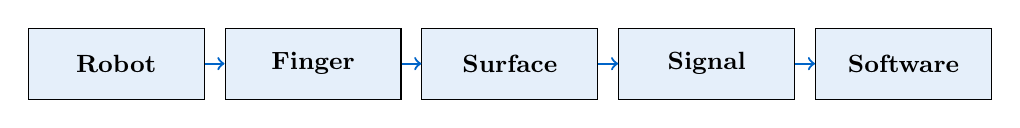
\begin{tikzpicture}[scale=1.0, node distance=1.6cm, every node/.style={font=\small}]
    
    % === Upper line – 5 boxes ===
    \node[draw,fill=primaryblue!10,minimum height=0.9cm,text width=2cm,align=center] (u1) at (0.5,4) {\textbf{Robot}};
    \node[draw,fill=primaryblue!10,minimum height=0.9cm,text width=2cm,align=center] (u2) at (3,4) {\textbf{Finger}};
    \node[draw,fill=primaryblue!10,minimum height=0.9cm,text width=2cm,align=center] (u3) at (5.5,4) {\textbf{Surface}};
    \node[draw,fill=primaryblue!10,minimum height=0.9cm,text width=2cm,align=center] (u4) at (8,4) {\textbf{Signal}};
    \node[draw,fill=primaryblue!10,minimum height=0.9cm,text width=2cm,align=center] (u5) at (10.5,4) {\textbf{Software}};
    
    \draw[->,thick,primaryblue] (u1) -> (u2);
    \draw[->,thick,primaryblue] (u2) -> (u3);
    \draw[->,thick,primaryblue] (u3) -> (u4);
    \draw[->,thick,primaryblue] (u4) -> (u5);
\end{tikzpicture}
\end{frame}


\begin{frame}{End-to-end Project Pipeline}

\begin{center}
\textbf{Core Process + Iterative Improvement}
\end{center}

\vspace{0.5cm}

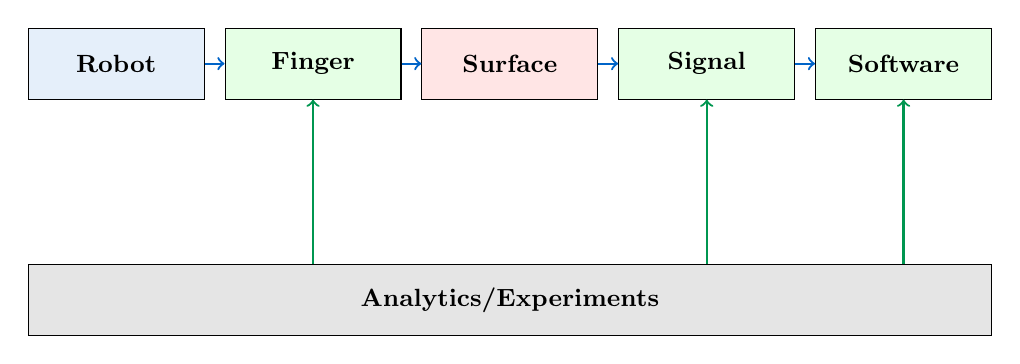
\begin{tikzpicture}[scale=1.0, node distance=1.6cm, every node/.style={font=\small}]
    
    % === Upper line – 5 boxes ===
    \node[draw,fill=primaryblue!10,minimum height=0.9cm,text width=2cm,align=center] (u1) at (0.5,4) {\textbf{Robot}};
    \node[draw,fill=green!10,minimum height=0.9cm,text width=2cm,align=center] (u2) at (3,4) {\textbf{Finger}};
    \node[draw,fill=red!10,minimum height=0.9cm,text width=2cm,align=center] (u3) at (5.5,4) {\textbf{Surface}};
    \node[draw,fill=green!10,minimum height=0.9cm,text width=2cm,align=center] (u4) at (8,4) {\textbf{Signal}};
    \node[draw,fill=green!10,minimum height=0.9cm,text width=2cm,align=center] (u5) at (10.5,4) {\textbf{Software}};
    
    \draw[->,thick,primaryblue] (u1) -> (u2);
    \draw[->,thick,primaryblue] (u2) -> (u3);
    \draw[->,thick,primaryblue] (u3) -> (u4);
    \draw[->,thick,primaryblue] (u4) -> (u5);
    
    
    % === Lower line – One wide box ===
    \node[draw,fill=gray!20,minimum height=0.9cm,text width=12cm,align=center] (l1) at (5.5,1) {\textbf{Analytics/Experiments}};
    
    
    % === Arrows from lower to upper ===
    \draw[->,thick,successgreen] (u2 |- l1.north) -> (u2.south);
    \draw[->,thick,successgreen] (u4 |- l1.north) -> (u4.south);
    \draw[->,thick,successgreen] (u5 |- l1.north) -> (u5.south);
\end{tikzpicture}
\end{frame}

% Research Question
\begin{frame}{Research Question}
\begin{center}
\Large How can we achieve geometrical reconstruction of complex 3D shapes using acoustic tactile sensing?
\end{center}

\vspace{0.5cm}

\textbf{Sub-Questions:}
\begin{itemize}
    \item \textbf{Can we distinguish between different contact scenarios?}
    \item \textbf{Which models perform the best on our datasets?}
    \item \textbf{What information can be extracted from acoustic responses?}
    \item \textbf{What information should we focus on?}
    \item \textbf{Which Frequencies Matter the Most?}
\end{itemize}

\end{frame}

% Datasets
\begin{frame}{Datasets}
\begin{table}
\centering
\begin{tabular}{|l|l|c|c|}
\hline
\textbf{Dataset} & \textbf{Contact Type} & \textbf{Classes} & \textbf{Samples} \\
\hline
Batch 1 & Position detection & 4 & 200 \\
Batch 2 & Position detection & 4 & 200 \\
Batch 3 & Edge detection (simple) & 3 & 150 \\
Batch 4 & Paper clip detection & 2 & 100 \\
Edge v1 & Edge detection (complex) & 3 & 630 \\
\hline
\textbf{Total} & & \textbf{2-4} & \textbf{1,280} \\
\hline
\end{tabular}
\end{table}

\vspace{0.5cm}
Batches 1-4 have 50 samples per class. Edge v1 has 210 samples per class.
\end{frame}

% ──────────────────────────────────────────────────────────────
% CLEAN DIMENSIONALITY REDUCTION SLIDE (exactly what you wanted)
% ──────────────────────────────────────────────────────────────
\begin{frame}{Dimensionality Reduction - Batch 2}

\textbf{Can we distinguish between different contact scenarios?} 
\vspace{0.8cm}

\begin{columns}

\begin{column}{0.5\textwidth}
\textbf{PCA Analysis}
\begin{center}
\includegraphics[width=\textwidth]{soft_finger_batch_2_pca_analysis.png}
\end{center}
\end{column}

\begin{column}{0.5\textwidth}
\textbf{t-SNE Analysis}
\begin{center}
\includegraphics[width=\textwidth]{soft_finger_batch_2_tsne_perplexity_50.png}
\end{center}
\end{column}

\end{columns}

\end{frame}

% ──────────────────────────────────────────────────────────────
% CLASSIFIER COMPARISON – CLEAN & PROFESSIONAL
% ──────────────────────────────────────────────────────────────
\begin{frame}{Classification Performance}

\textbf{Which models perform the best on our datasets?}

\vspace{0.5cm}

\textbf{Tested Classifiers:}
\begin{itemize}
    \item \textbf{Random Forest} – Combines many decision trees to make smarter predictions
    \item \textbf{SVM (RBF)} – Draws the best curved boundary to separate different classes
    \item \textbf{SVM (Linear)} – Draws a straight line to separate different classes
    \item \textbf{K-Nearest Neighbors} – Classifies based on the majority vote of nearby similar examples
    \item \textbf{Logistic Regression} – Predicts probabilities using a straight-line relationship
    \item \textbf{Gradient Boosting} – Builds trees one by one, each fixing the mistakes of the previous
    \item \textbf{Linear Discriminant Analysis} – Finds the best direction to tell classes apart
\end{itemize}

\end{frame}

\begin{frame}{Model Performance - Batch 2}

\begin{center}
\includegraphics[width=\textwidth]{soft_finger_batch_2_classifier_performance.png}
\end{center}

\end{frame}
% ──────────────────────────────────────────────────────────────
% WHAT INFORMATION CAN WE EXTRACT FROM ACOUSTIC RESPONSES?
% ──────────────────────────────────────────────────────────────
\begin{frame}{What information can be extracted from acoustic responses?}

\textbf{1. Direct Signal Analysis}
\begin{itemize}
    \item \textbf{Waveform}: overall energy, fade over time
    \item \textbf{Frequency Spectrum}: center, bandwidth
    \item \textbf{Time-Frequency View}: freq changes, spectrum contrasts
    \item \textbf{High Frequencies}: energy ratio above 8 kHz
\end{itemize}

\vspace{0.5cm}

\textbf{2. System Response Analysis (Transfer Function)}
\begin{itemize}
    \item \textbf{Signal Separation} $H(f) = Y(f)/X(f)$ → true system behavior
    \item \textbf{Peak Frequencies}: peak amplitude, peak frequency location
    \item \textbf{Frequency Stats}: Q-factor, asymmetry
\end{itemize}
\end{frame}

% Slide with question: What information should we focus on?
\begin{frame}{What information should we focus on?}
\textbf{How Feature Ablation Works:}
\begin{itemize}
    \item Remove one feature at a time and retrain
    \item Measure accuracy drop
\end{itemize}

\vspace{0.5cm}

\textbf{Main Finding:}
\begin{itemize}
    \item Subsets of features can be used across all datasets
\end{itemize}

\begin{table}[h]
\centering
\scriptsize
\begin{tabular}{|l|c|c|c|c|c|}
\hline
\textbf{Dataset} & \textbf{Baseline} & \textbf{Optimal} & \textbf{Optimal Acc.} & \textbf{Max Drop} & \textbf{Increase Ex.} \\
\hline
Batch 1 & 96\% & 2/38 & 99\% & 1.0\% & Feature 35 (+0.5\%) \\
Batch 2 & 99.5\% & 10/38 & 99.5\% & 1.5\% & None \\
Batch 3 & 99.3\% & 1/38 & 100\% & 1.3\% & None \\
Batch 4 & 85\% & 10/38 & 86\% & 2.1\% & None \\
Edge v1 & 66\% & 13/38 & 71\% & 5.6\% & Feature 11 (+0.8\%) \\
\hline
\end{tabular}
\end{table}

\end{frame}

% ──────────────────────────────────────────────────────────────
% OPTIMAL FEATURE SUBSETS
% ──────────────────────────────────────────────────────────────
\begin{frame}{What information should we focus on?}
\begin{table}[h]
\centering
\scriptsize
\begin{tabular}{|l|p{10cm}|}
\hline
\textbf{Dataset} & \textbf{Optimal Features} \\
\hline
Batch 1 & ultra\_high\_energy\_ratio, spectral\_bandwidth, ultra\_high\_ratio, high\_energy\_ratio, spectral\_centroid, mid\_energy\_ratio, spectral\_flatness, env\_skew, low\_mid\_ratio, env\_kurtosis, high\_freq\_decay\_rate \\
Batch 2 & spectral\_centroid, ultra\_high\_energy\_ratio, high\_energy\_ratio, ultra\_high\_ratio, low\_mid\_ratio, mid\_energy\_ratio, burst\_rms, env\_kurtosis, env\_skew, temporal\_centroid, damping\_ratio \\
Batch 3 & spectral\_bandwidth, high\_energy\_ratio, spectral\_centroid, ultra\_high\_energy\_ratio, mid\_energy\_ratio, ultra\_high\_ratio, low\_mid\_ratio, damping\_ratio, spectral\_flatness, resonance\_high\_ratio, high\_freq\_slope \\
Batch 4 & env\_std, burst\_rms, env\_mean, resonance\_energy\_ratio, spectral\_bandwidth, temporal\_centroid, spectral\_centroid, low\_mid\_ratio, env\_kurtosis, spectral\_flatness, env\_max \\
Edge v1 & spectral\_bandwidth, ultra\_high\_energy\_ratio, spectral\_centroid, ultra\_high\_ratio, high\_energy\_ratio, env\_skew, env\_kurtosis, spectral\_flatness, burst\_rms, resonance\_skewness, low\_mid\_ratio \\
\hline
\end{tabular}
\end{table}

\begin{table}[h]
\centering
\scriptsize
\begin{tabular}{|l|p{10cm}|}
\hline
\textbf{Dataset} & \textbf{Features Improving When Removed} \\
\hline
Batch 1 & high\_freq\_slope, spectral\_contrast\_0, spectral\_contrast\_1, spectral\_contrast\_2, spectral\_contrast\_3, spectral\_contrast\_4 etc. \\
Edge v1 & resonance\_skewness, resonance\_q\_factor \\
\hline
\end{tabular}
\end{table}

\end{frame}

% Experiment 4
\begin{frame}{What information should we focus on?}

\textbf{Saliency Analysis:} Analyze which features neural networks consider most important for classification decisions.

\textbf{Method:}
\begin{itemize}
    \item Train neural networks on each dataset using all 38 features
    \item Apply gradient-based saliency to rank feature importance
    \item Identify top features influencing NN predictions
\end{itemize}

\textbf{Results - NN Performance and Feature Importance:}
\begin{table}[h]
\centering
\scriptsize
\begin{tabular}{|l|c|p{6cm}|}
\hline
\textbf{Dataset} & \textbf{NN Accuracy} & \textbf{Top 5 Features} \\
\hline
Batch 1 & 95\% & spectral\_bandwidth, resonance\_skewness, spectral\_centroid, ultra\_high\_ratio, zero\_crossing\_rate \\
Batch 2 & 93\% & env\_min, resonance\_high\_ratio, damping\_ratio, zero\_crossing\_rate, ultra\_high\_ratio \\
Batch 3 & 97\% & spectral\_bandwidth, env\_decay\_rate, spectral\_centroid, resonance\_q\_factor, env\_mean \\
Batch 4 & 80\% & resonance\_skewness, spectral\_contrast\_4, env\_std, spectral\_centroid, spectral\_bandwidth \\
Edge v1 & 54\% & ultra\_high\_energy\_ratio, ultra\_high\_ratio, spectral\_bandwidth, spectral\_flatness, high\_energy\_ratio \\
\hline
\end{tabular}
\end{table}
\end{frame}

% ──────────────────────────────────────────────────────────────
% FREQUENCY ABLATION EXPERIMENT - SLIDE 1
% ──────────────────────────────────────────────────────────────
\begin{frame}{Which Frequencies Matter the Most?}

\textbf{Question:} Which frequency ranges contain the most useful information for classifying contact types?

\vspace{1.0cm}

\textbf{What We Tested:}
\begin{itemize}
    \item 12 different frequency bands (20Hz to 20kHz)
    \item 5 datasets with different contact scenarios
    \item Random Forest classifier performance
\end{itemize}
\end{frame}

% ──────────────────────────────────────────────────────────────
% FREQUENCY ABLATION EXPERIMENT - SLIDE 2
% ──────────────────────────────────────────────────────────────
\begin{frame}{Which Frequencies Matter the Most?}

\begin{table}[h]
\centering
\scriptsize
\begin{tabular}{|l|c|c|c|c|c|}
\hline
\textbf{Band} & \textbf{edge\_v1} & \textbf{batch\_1} & \textbf{batch\_2} & \textbf{batch\_3} & \textbf{batch\_4} \\
\hline
20-200Hz & \cellcolor{errorred!20}33.3\% & \cellcolor{errorred!20}25.0\% & \cellcolor{errorred!20}25.0\% & \cellcolor{errorred!20}33.3\% & \cellcolor{errorred!20}50.0\% \\
200-500Hz & 40.0\% & 90.0\% & \cellcolor{errorred!20}94.0\% & \cellcolor{errorred!20}68.7\% & \cellcolor{errorred!20}63.0\% \\
500-1000Hz & \cellcolor{errorred!20}35.2\% & \cellcolor{errorred!20}70.5\% & \cellcolor{errorred!20}94.5\% & 90.7\% & 66.0\% \\
1000-2000Hz & \cellcolor{errorred!20}33.0\% & 80.5\% & \cellcolor{errorred!20}94.5\% & 94.7\% & 70.0\% \\
2000-4000Hz & 38.7\% & 82.5\% & \cellcolor{green!20}\textbf{99.5\%} & \cellcolor{green!20}\textbf{99.3\%} & 69.0\% \\
4000-8000Hz & 45.2\% & 86.5\% & \cellcolor{green!20}\textbf{99.0\%} & \cellcolor{green!20}\textbf{100.0\%} & \cellcolor{green!20}\textbf{78.0\%} \\
8000-20000Hz & \cellcolor{green!20}\textbf{61.4\%} & \cellcolor{green!20}\textbf{96.0\%} & \cellcolor{green!20}\textbf{99.5\%} & \cellcolor{green!20}\textbf{100.0\%} & 74.0\% \\
\arrayrulecolor{red}\hline\arrayrulecolor{black}
20-20000Hz & \cellcolor{yellow!20}59.2\% & \cellcolor{yellow!20}94.5\% & \cellcolor{yellow!20}100.0\% & \cellcolor{yellow!20}99.3\% & \cellcolor{yellow!20}84.0\% \\
\hline
\end{tabular}
\end{table}

\vspace{0.3cm}
\textbf{Color Coding:}
\begin{itemize}
    \item \colorbox{green!20}{Green}: Top 3 performers per dataset
    \item \colorbox{yellow!20}{Yellow}: Full spectrum baseline (20-20000Hz)
    \item \colorbox{errorred!20}{Red}: Bottom 3 performers per dataset
\end{itemize}

\end{frame}

% ──────────────────────────────────────────────────────────────
% FINAL CONCLUSION – SHORT, STRONG, MEMORABLE (one slide only)
% ──────────────────────────────────────────────────────────────
\begin{frame}{Conclusion \& Look Ahead}

\begin{alertblock}{Core Message}
\textbf{We should be able to perform geometrical reconstruction with our setup including two contact scenarios.}
\end{alertblock}

\vspace{0.5cm}

\textbf{Iterative improvement loop:}
\begin{enumerate}[1.]
    \item More complex surface / object $\rightarrow$ new data
    \item Analyze $\rightarrow$ discover what actually matters
    \item Improve finger, signal, or software
\end{enumerate}

\end{frame}

\end{document}